%====================================================================%
%                  MORIOND.TEX                                       %
%====================================================================%

\documentclass{moriond}


\bibliographystyle{unsrt}    
% for BibTeX - sorted numerical labels by order of
% first citation.

% A useful Journal macro
\def\Journal#1#2#3#4{{#1} {\bf #2}, #3 (#4)}

% Some useful journal names
\def\NCA{\em Nuovo Cimento}
\def\NIM{\em Nucl. Instrum. Methods}
\def\NIMA{{\em Nucl. Instrum. Methods} A}
\def\NPB{{\em Nucl. Phys.} B}
\def\PLB{{\em Phys. Lett.}  B}
\def\PRL{\em Phys. Rev. Lett.}
\def\PRD{{\em Phys. Rev.} D}
\def\ZPC{{\em Z. Phys.} C}

% Some other macros used in the sample text
\def\st{\scriptstyle}
\def\sst{\scriptscriptstyle}
\def\mco{\multicolumn}
\def\epp{\epsilon^{\prime}}
\def\vep{\varepsilon}
\def\ra{\rightarrow}
\def\ppg{\pi^+\pi^-\gamma}
\def\vp{{\bf p}}
\def\ko{K^0}
\def\kb{\bar{K^0}}
\def\al{\alpha}
\def\ab{\bar{\alpha}}
\def\be{\begin{equation}}
\def\ee{\end{equation}}
\def\bea{\begin{eqnarray}}
\def\eea{\end{eqnarray}}
\def\CPbar{\hbox{{\rm CP}\hskip-1.80em{/}}}
%temp replacement due to no font
%%%%%%%%%%%%%%%%%%%%%%%%%%%%%%%%%%%%%%%%%%%%%%%%%%
%                                                %
%    BEGINNING OF TEXT                           %
%                                                %
%%%%%%%%%%%%%%%%%%%%%%%%%%%%%%%%%%%%%%%%%%%%%%%%%%

\newcommand{\Photo}{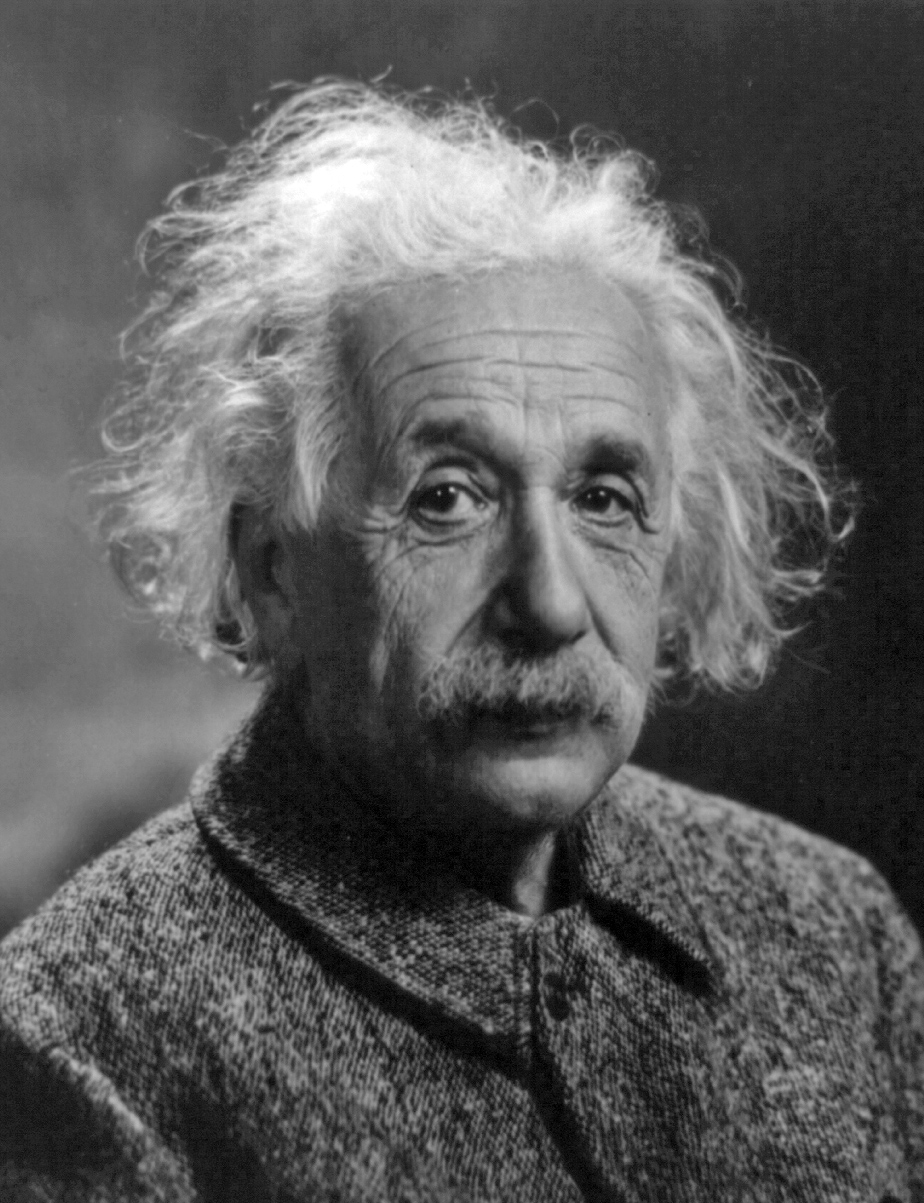
\includegraphics[height=35mm]{mypicture}}
%\newcommand{\Photo}{}

\begin{document}
\vspace*{4cm}
\title{Highlights of ATLAS Search Results}


\author{Bingxuan Liu, on behalf of the ATLAS Collaboration}

\address{Department of Physics, Simon Fraser University, Vancouver, Canada}

\maketitle\abstracts{Searching for beyond standard model (BSM) physics has been
one of the primary goals of the LHC physics program. The LHC delivered 140
$\mathrm{fb}^{-1}$ data of high quality in Run 2, allowing both the ATLAS and
CMS collaborations to expand and improve their search programs. The recent
development in detector perforamnce and analysis techniques have brought
significant boosts to the search sensitivities. In this article, highlights of
recent ATLAS search results are discussed and summarized.}  

\section{Introduction}

\section*{References}

\begin{thebibliography}{99}
\bibitem{ja}C Jarlskog in {\em CP Violation}, ed. C Jarlskog
(World Scientific, Singapore, 1988).

\bibitem{ma}L. Maiani, \Journal{\PLB}{62}{183}{1976}.

\bibitem{bu}J.D. Bjorken and I. Dunietz, \Journal{\PRD}{36}{2109}{1987}.

\bibitem{bd}C.D. Buchanan {\it et al}, \Journal{\PRD}{45}{4088}{1992}.

\end{thebibliography}

\end{document}

%%%%%%%%%%%%%%%%%%%%%%
% End of moriond.tex  %
%%%%%%%%%%%%%%%%%%%%%%


%%% Local Variables: 
%%% mode: latex
%%% TeX-master: t
%%% End: 

%%% Local Variables: 
%%% mode: latex
%%% TeX-master: t
%%% End: 

%%% Local Variables: 
%%% mode: latex
%%% TeX-master: t
%%% End: 
